%-----------------------------------------------------------------------------------------------
\section{Evaluation}
\subsection{Design}
\begin{frame}
\frametitle{Research Design - Data Structure} 
\begin{itemize}
	\item \textbf{3 cities - Reggio, Parma and Padova}
	\begin{itemize}
		\item Similar geographic location
		\item Parma more similar to Reggio in terms of culture and history
	\end{itemize}
	\bigskip
	\item \textbf{5 cohorts - Ages 6, 17, 30, 40 \&  50}
	\begin{itemize}
		\item Age 6: Children entering elementary school
		\item Age 17: Adolescents reaching maturity
		\item Age 31-32: Adults at first life milestone
		\item Age 40-41: Adults at second milestone. First to get access to ITC
		\item Age 53-58: Adults born before RCA was implemented
	\end{itemize}
\end{itemize}
\end{frame} 

%-----------------------------------------------------------------------------------------------
\begin{frame}
\frametitle{Reggio Emilia, Parma, Padova} 
\begin{center}
\begin{figure}
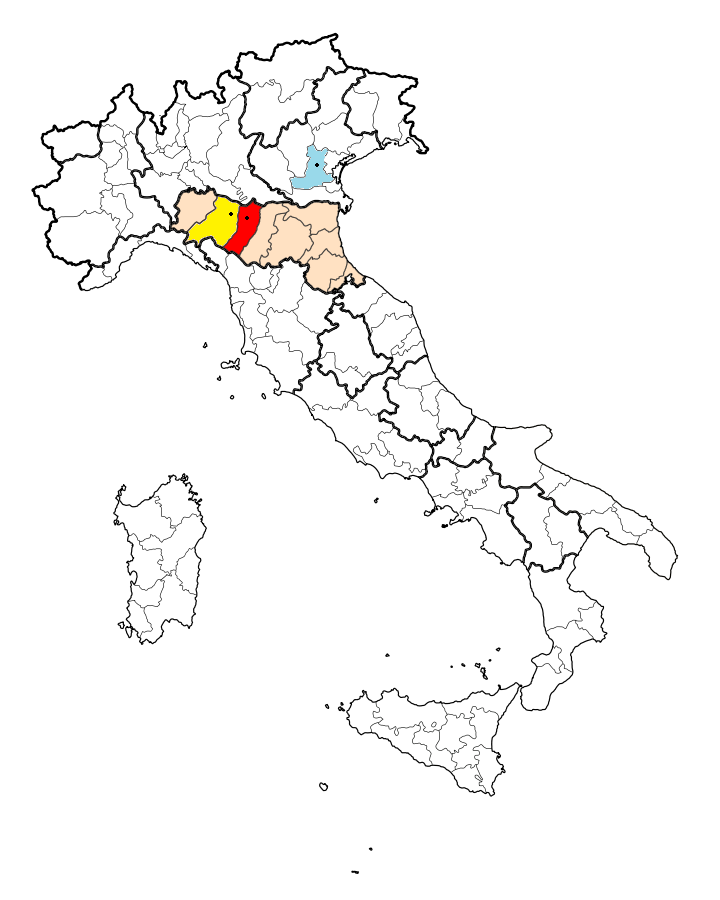
\includegraphics[height=1.0\textheight]{include/3-cities-map.png}
%\caption{{Location of the city of Parma, Reggio Emilia, and Padova, Italy.}}
\end{figure}
\end{center}
\end{frame}
%-----------------------------------------------------------------------------------------------
\begin{frame} 
\frametitle{Sample by City and Cohort}
\begin{figure}[H]
\begin{center}
	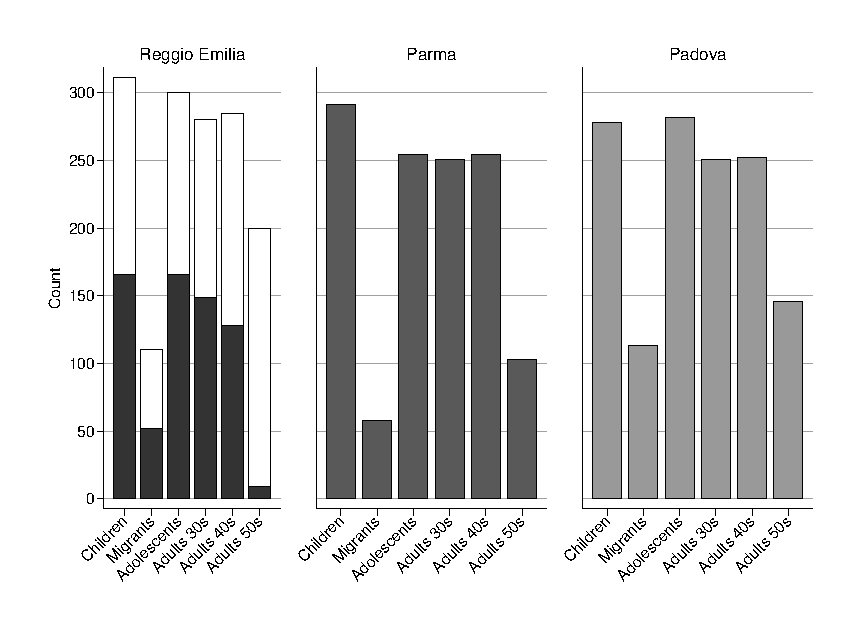
\includegraphics[width=.8\textwidth]{./include/sample}
\end{center}
\footnotetext{\scriptsize \noindent \textit{Note}: Number of individuals by cohort and city. In Reggio Emilia we differentiate between those who attended municipal preschool (black bars) and those who did not (white bars).}
\end{figure}
\end{frame}
%%-----------------------------------------------------------------------------------------------
\begin{frame}
\frametitle{Attendance Infant-toddler Centers (0-3)} 
\begin{center}
\begin{figure}
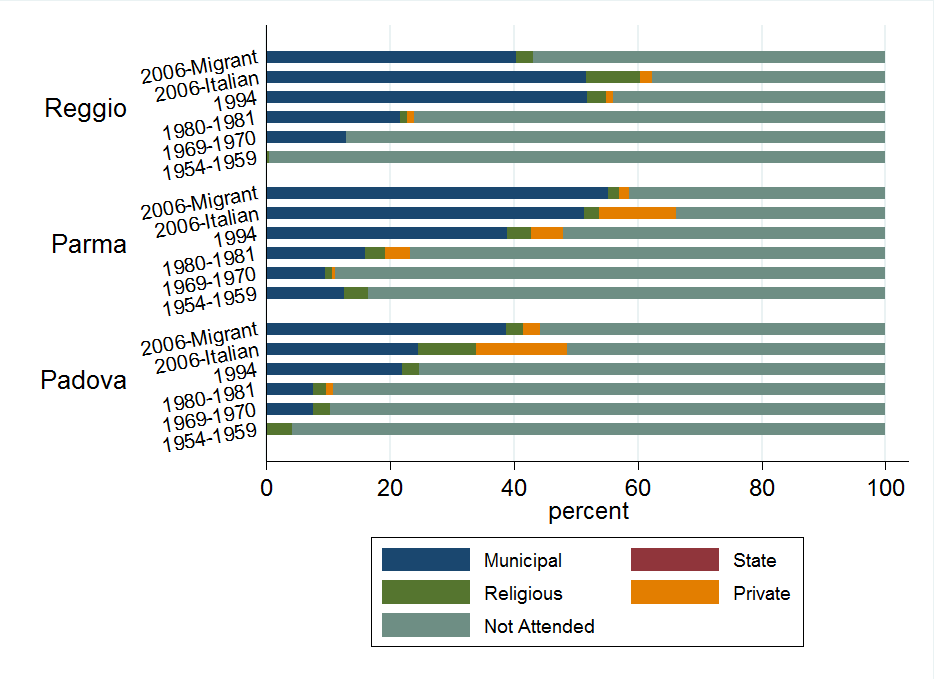
\includegraphics[width=1.15\textheight]{asiloType-Attend.png}
%\caption{{Location of the city of Parma, Reggio Emilia, and Padova, Italy.}}
\end{figure}
\end{center}
\end{frame}
%------------------------------------------------------------------------------------------------
\begin{frame}
\frametitle{Attendance Preschools (3-6)} 
\begin{center}
\begin{figure}
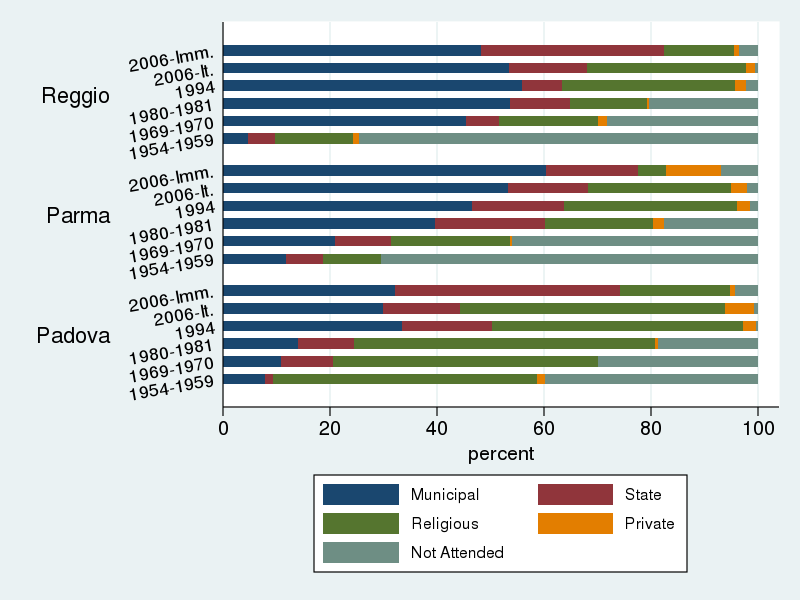
\includegraphics[width=1.15\textheight]{maternaType-Attend.png}
%\caption{{Location of the city of Parma, Reggio Emilia, and Padova, Italy.}}
\end{figure}
\end{center}
\end{frame}
%-------------------------------------------------------------------------------------------------
\begin{frame}
\frametitle{Research Design -Treatment} 
\underline{\textbf{Definition of Treatment}}
\begin{itemize}
	\item \textbf{Treated:} Those who attended Municipal schools in Reggio
	\smallskip
	\item \textbf{Control:} Those who didn't attend Municipal schools in Reggio
	\begin{itemize}
		\item Attended non-Municipal schools in Reggio
		\item Attended any school in Parma or Padova
		\item Attended no preschool in any city
	\end{itemize}
\end{itemize}
\bigskip
\underline{\textbf{Potential Issues:}}
\begin{itemize}
	\item Diffusion of Reggio Approach into control group
	\item Differential rates of diffusion over time, between schools, and across cities
\end{itemize}
\begin{block}{}
$\mathbf{\hookrightarrow}$ Recently conducted interviews to understand these differences
\end{block}

\end{frame}
%-----------------------------------------------------------------------------------------------